\documentclass[11pt,letterpaper]{article}
\usepackage[utf8]{inputenc}
\usepackage[margin=1in]{geometry}
\usepackage{amsmath}
\usepackage{amsfonts}
\usepackage{amssymb}
\usepackage{amsthm}
\usepackage{verbatim}
\usepackage{graphicx}
% No paragraph tabs
\setlength{\parindent}{0pt}

% Define commands that will be widely used.
\newcommand{\br}{\ \\}
\newcommand{\tab}{\hspace*{2em}}

\title{EAX Assignment}
\author{Rachel Domagalski}
\date{September 10, 2013}

\begin{document}
\maketitle

\section*{Problem 1}

When counting events in a given time interval, the distribution of the counts is
Poisson. Since the standard deviation on a Poisson distribution is $\sqrt{N}$,
the relative precision on a measurement is $\dfrac{1}{\sqrt{N}}$. To get a
precision of 2\%, 2500 counts will be needed. Given that it takes 10 minutes to
record 2000 counts, it will take 12.5 minutes to get record 2500 counts and thus
get a precision of 2\%.

\section*{Problem 2}

It is assumed in all of these exercises that the errors on $A$ and $B$ are
uncorrelated.

\begin{description}
\item[A] \hfill \\
    When adding two measurements, the variance is
    \begin{displaymath}
        \sigma_{A+B}^2 = \frac{1}{NM} \sum_{i=1}^N \sum_{j=1}^M
        \left(\left(A_i + B_j\right) - \left(\mu_A + \mu_B\right)\right)^2 =
        \frac{1}{NM} \sum_{i=1}^N \sum_{j=1}^M
        \left(\left(A_i - \mu_A\right) + \left(B_j - \mu_B\right)\right)^2
    \end{displaymath}
    This rearranges to
    \begin{equation}
        \sigma_{A+B}^2 = \frac{1}{NM} \sum_{i=1}^N \sum_{j=1}^M \left[
        \left(A_i - \mu_A\right)^2 + \left(B_j - \mu_B\right)^2 +
        2\left(A_i - \mu_A\right) \left(B_j - \mu_B\right) \right]
        \label{sumsigma}
    \end{equation}
    This reduces to
    \begin{displaymath}
        \sigma_{A+B}^2 =
        \sigma_A^2 + \sigma_B^2 + \frac{2}{NM} \sum_{i=1}^N \sum_{j=1}^M
        \left(A_i - \mu_A\right) \left(B_j - \mu_B\right)
    \end{displaymath}
    The third term on the right hand side can be canceled as the difference
    between the computed mean and expected mean of a set of data goes to zero.
    From this, the variance of adding to measurements can be computed as
    \begin{equation}
        \sigma_{A+B}^2 = \sigma_A^2 + \sigma_B^2
        \label{sumerr}
    \end{equation}
\item[B] \hfill \\
    The argument for subtracting two measurements is pretty much identical to
    adding two measurements, except that the $2\left(A_i - \mu_A\right)
    \left(B_i - \mu_B\right)$ term in \eqref{sumsigma} will have a minus sign in
    front. Therefore, the variance for subtracting two measurements is given by
    \eqref{sumerr}.
\item[C] \hfill \\
    The error for $2A + 2B$ is the twice the error of $A + B$, as $\sigma$ will
    scale linearly.
    \begin{equation}
    \sigma_{2A + 2B} = 2 \sqrt{\sigma_A^2 + \sigma_B^2}
    \end{equation}
\item[D] \hfill \\
    Let $f = A^m B^n$. From this, we get $df = \left(\dfrac{\partial f}{\partial
    A}\right)dA + \left(\dfrac{\partial f}{\partial B}\right) dB$. Since
    $\dfrac{\partial f}{\partial A} = mA^{m-1}$ and $\dfrac{\partial f}{\partial
    B} = nB^{n-1}$, we get
    \begin{equation}
        \dfrac{\delta f}{f} = m \dfrac{\delta A}{A} + n \dfrac{\delta B}{B}
        \label{deltaprod}
    \end{equation}
    Like with summing or subtracting errors, \eqref{deltaprod} can be squared
    and averaged.
    \begin{displaymath}
        \left(\frac{\sigma_f}{f}\right)^2 = \left(m\frac{\sigma_A}{A}\right)^2 +
        \left(n\frac{\sigma_B}{B}\right)^2 + \frac{2mn}{MN} \sum_{i=1}^{M}
        \sum_{j=1}^{N} \frac{\delta A_i}{A_i} \frac{\delta B_j}{B_j}
    \end{displaymath}
    As before, the last term on the right hand side will average out to zero,
    giving the expression for the variance of products.
    \begin{equation}
        \left(\frac{\sigma_f}{f}\right)^2 = m^2\left(\frac{\sigma_A}{A}\right)^2
        + n^2 \left(\frac{\sigma_B}{B}\right)^2
        \label{varprod}
    \end{equation}
    In the specific case of $m = n = 1$, \eqref{varprod} reduces to
    \begin{displaymath}
        \left(\frac{\sigma_{AB}}{AB}\right)^2 =
        \left(\frac{\sigma_A}{A}\right)^2 + \left(\frac{\sigma_B}{B}\right)^2
    \end{displaymath}
    and the variance of a product of two measurements $A$ and $B$ becomes
    \begin{equation}
        \sigma_{AB}^2 = B^2 \sigma_A^2 + A^2 \sigma_B^2
    \end{equation}

\end{description}

\section*{Problem 3}

The random number generator that was passed to the GNU Scientific Library (GSL)
function for sampling from a Gaussian was the Mersenne-Twister MT19937, seeded
by the system time, which is the number of seconds from January 1, 1970. For
more information, consult the GSL manual as well as the man page for the C
header file time.h, which should be available on most Unix systems. All other
details for the code that was used to complete this assignment can be found at
https://bitbucket.org/domagalski/physics111-advanced-lab/.

% Sampling 5 times from a gaussian
\begin{figure}
    \centering
    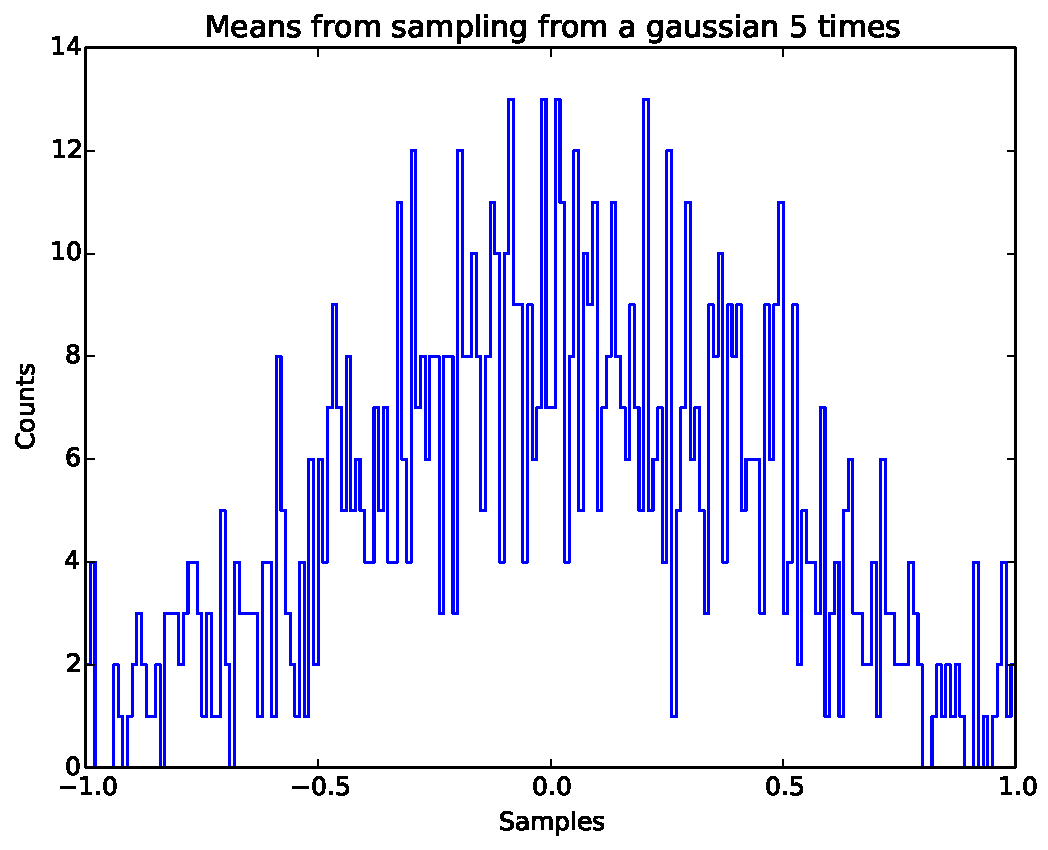
\includegraphics[width=0.6\textwidth]{figures/problem3_1.pdf}
    \caption{Gaussian sampling test using lists 5 elements.}
    \label{prob3_1}
\end{figure}

\begin{enumerate}
\item The expected mean and standard deviation when sampling from a normal
    distribution is 0 and 1 and this does not depend on the number of samples.
    The error of the mean of a Gaussian is $\dfrac{\sigma}{\sqrt{N}}$, so in the
    case of a normal distribution sampled 5 times, the expected error on the
    mean is approximately  $\dfrac{1}{\sqrt{5}} \approx 0.447$.
\item Using an sample list of length 5, an estimate of the mean of a Gaussian is
    0.0933852. The estimate of the standard deviation of this list is 1.15499
    and the error on the mean is 0.516526. Of course, due to the low number of
    samples, repetitions of this experiment could yield very different results.
    This is very different from the correct mean of the normal distribution, but
    the true mean is within the error on the sampled mean.
\item When running the previous sampling experiment 1000 times, the mean of all
    means was found to be $-8.92144 \times 10^{-3}$ and the error on the mean
    was 0.45737. This is a lot closer to the true value of the mean and the
    error on the mean of a Gaussian. It is also found in this experiment that
    95.8\% of the means were within $\pm 2\sigma$ of the mean. This is pretty
    close to the expected value of 95\% of samples being within $\pm 2\sigma$.
    See Figure \ref{prob3_1} for the distribution of the means. When using only
    5 samples to compute the mean, the spread on the means is very large.
\item The previous problems were repeated with sample sizes of 10, 50, 100,
    and 1000. As can be seen in Figure \ref{sample_gaus}, the standard deviation
    of the means gets smaller as the sample size grows.
    \begin{itemize}
    \item Sample size of 10:\\
        Example list:\\
        Mean: 0.24497\\
        Standard deviation: 0.778638\\
        Error on the mean: 0.246227\\
        Expected error on the mean: 0.316228\\
        \ \\
        Sampling from 1000 Gaussians.\\
        Average mean: -0.00202297\\
        Sigma of all means: 0.31565\\
        Percentage of experiments within 2 sigma: 95.1\%\\
    \item Sample size of 50:\\
        Example list:\\
        Mean: 0.0597558\\
        Standard deviation: 1.13171\\
        Error on the mean: 0.160048\\
        Expected error on the mean: 0.141421\\
        %\ \\
        Sampling from 1000 Gaussians:\\
        Average mean: -0.00580967\\
        Sigma of all means: 0.137353\\
        Percentage of experiments within 2 sigma: 95.6\%\\
    \item Sample size of 100:\\
        Example list:\\
        Mean: -0.0720972\\
        Standard deviation: 0.917531\\
        Error on the mean: 0.0917351\\
        Expected error on the mean: 0.1\\
        \ \\
        Sampling from 1000 Gaussians:\\
        Average mean: -0.0014912\\
        Sigma of all means: 0.100824\\
        Percentage of experiments within 2 sigma: 95.9\%\\
    \item Sample size of 1000:\\
        Example list:\\
        Mean: -0.0319888\\
        Standard deviation: 1.03214\\
        Error on the mean: 0.0326391\\
        Expected error on the mean: 0.0316228\\
        \ \\
        Sampling from 1000 Gaussians:\\
        Average mean: 0.000327042\\
        Sigma of all means: 0.0312426\\
        Percentage of experiments within 2 sigma: 95.2\%\\
    \end{itemize}
\item Based on the sample calculations above, the error of the mean of a single
    list approaches the error of the mean of all lists as the number of samples
    increases.
\end{enumerate}

% All gaussian sampling experiments
\begin{figure}
    \centering
    \begin{minipage}[t]{0.45\textwidth}
        \centering
        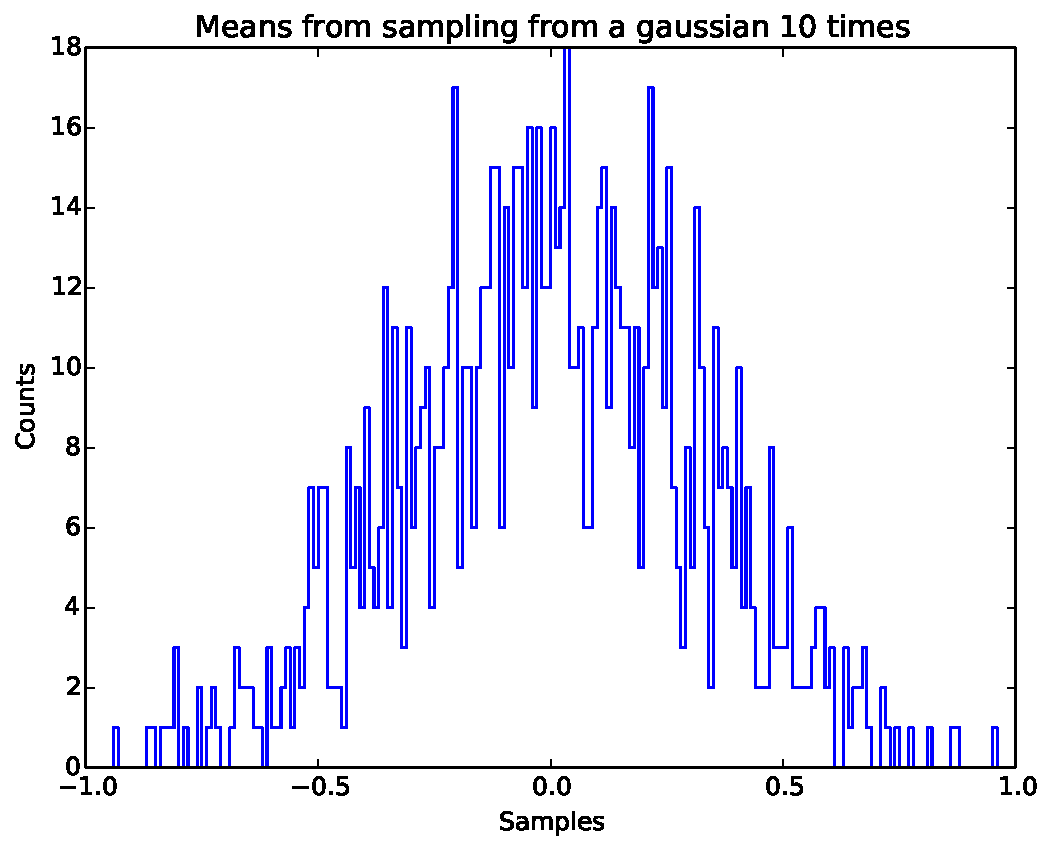
\includegraphics[width=\textwidth]{figures/problem3_2.pdf}
    \end{minipage}
    \hspace{0.5cm}
    \begin{minipage}[t]{0.45\textwidth}
        \centering
        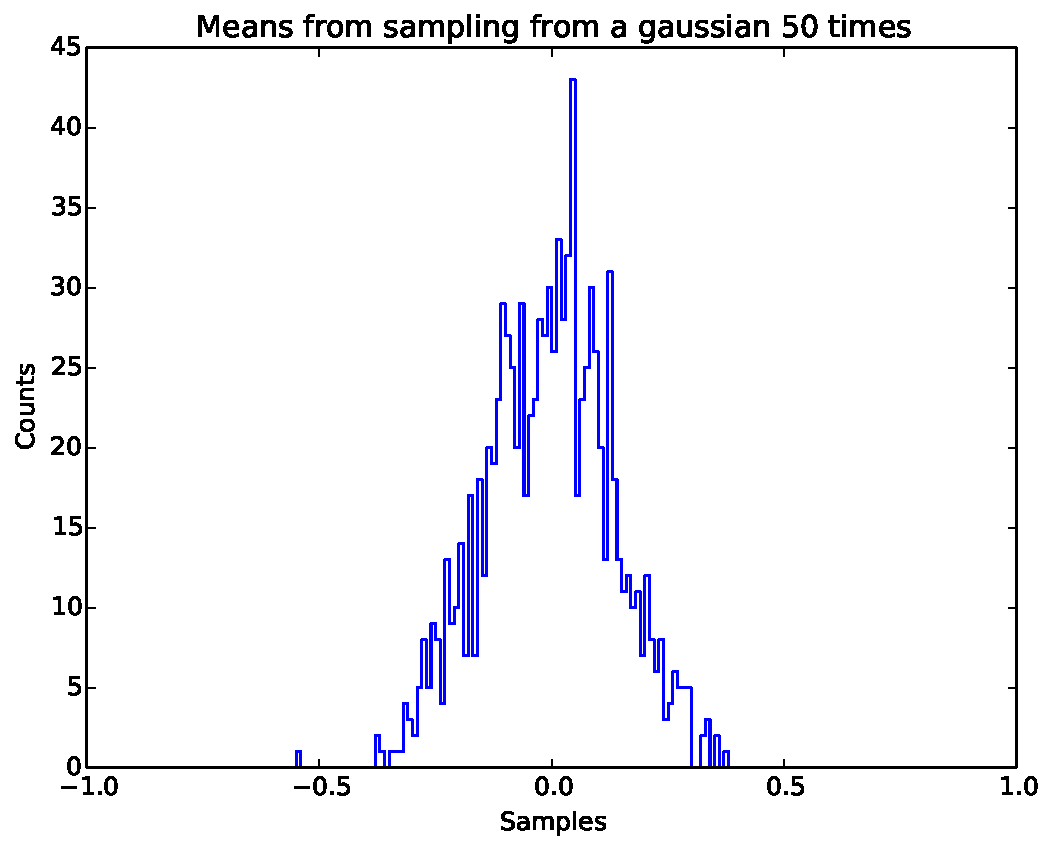
\includegraphics[width=\textwidth]{figures/problem3_3.pdf}
    \end{minipage}
    \begin{minipage}[t]{0.45\textwidth}
        \centering
        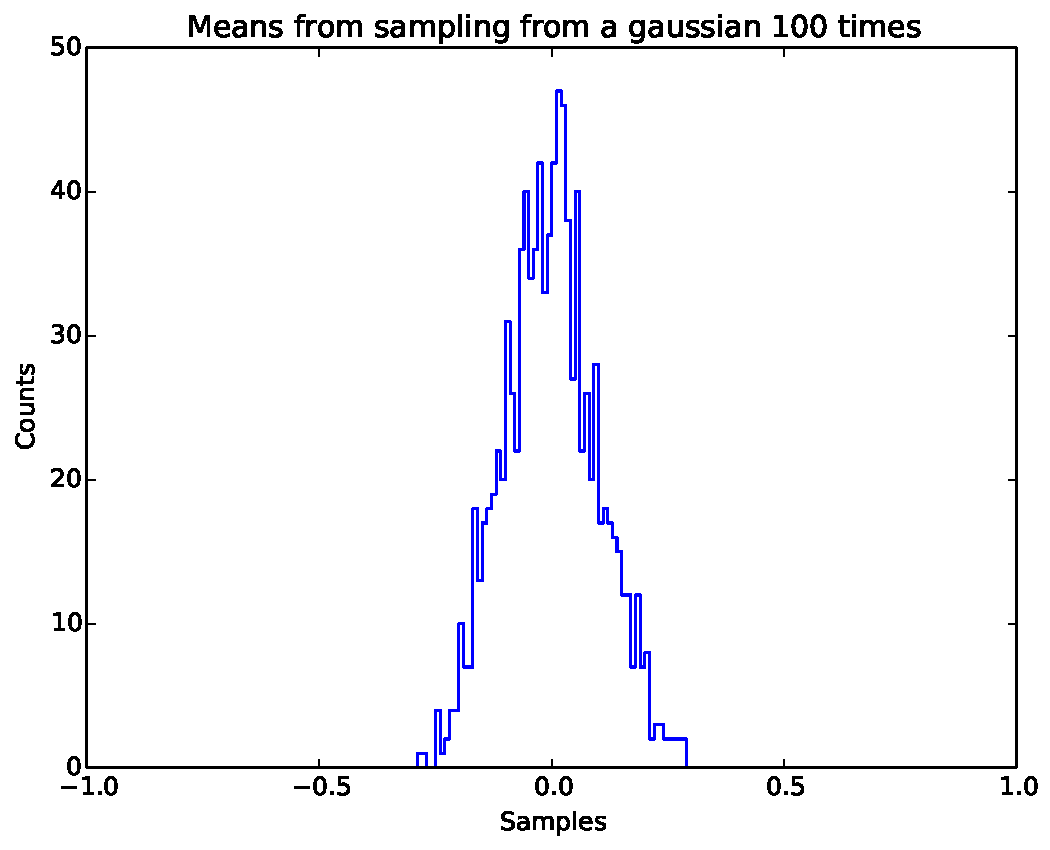
\includegraphics[width=\textwidth]{figures/problem3_4.pdf}
    \end{minipage}
    \hspace{0.5cm}
    \begin{minipage}[t]{0.45\textwidth}
        \centering
        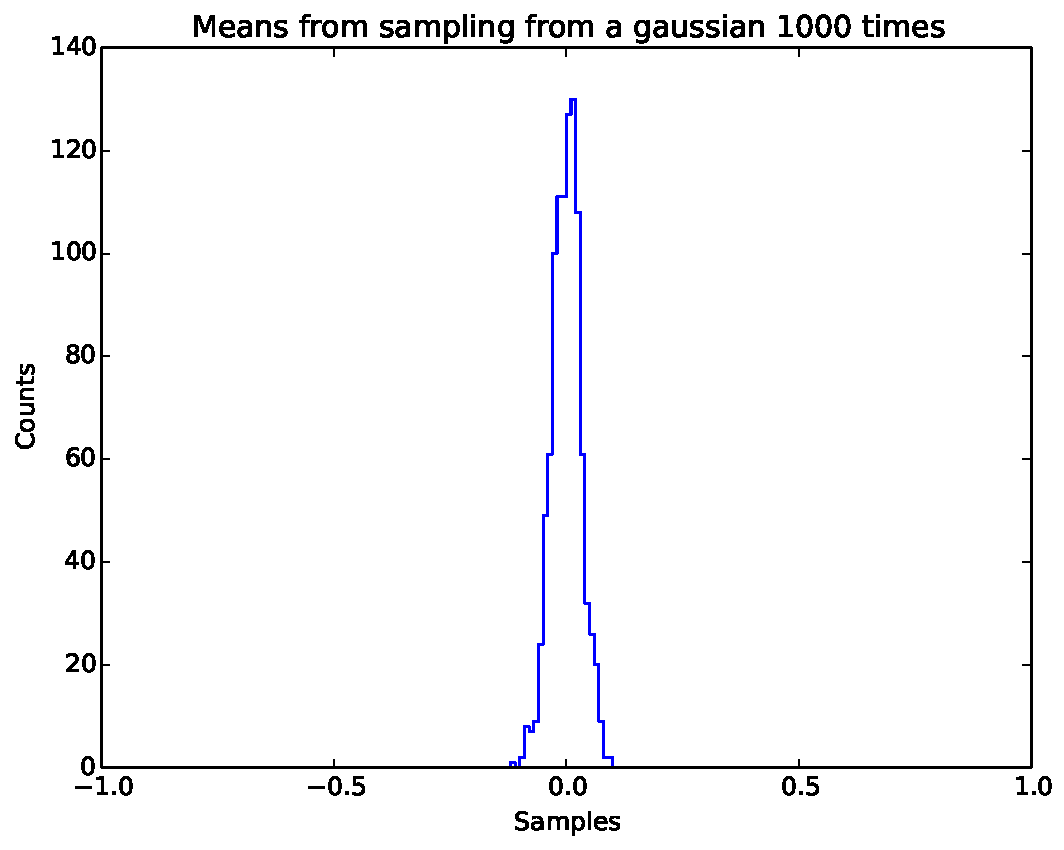
\includegraphics[width=\textwidth]{figures/problem3_5.pdf}
    \end{minipage}
    \caption{Gaussian sampling experiments for sample sizes of 10, 50, 100, and
    1000. The peak width on the distributions get smaller as the sample size
    gets larger.}
    \label{sample_gaus}
\end{figure}

% Gamma ray histogram
\begin{figure}
    \centering
    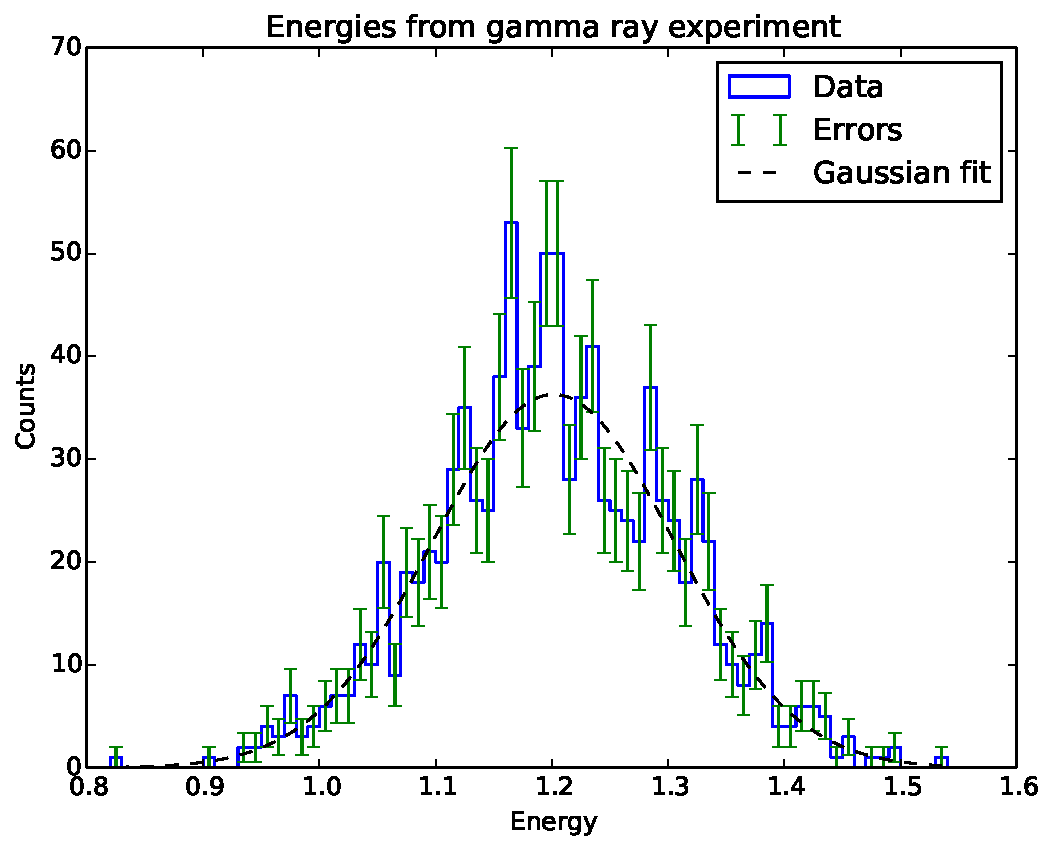
\includegraphics[width=0.7\textwidth]{figures/problem4.pdf}
    \caption{Distribution of energies from the gamma ray data.}
    \label{prob4}
\end{figure}

\section*{Problem 4}

\begin{enumerate}
\item See Figure \ref{prob4} for the distribution of energies, along with a
    Gaussian fit and error bars.
\item The mean and standard deviation computed directly from the data was
    1.203 and 0.104 respectively. The uncertainties on the mean and standard
    deviation are $\dfrac{\sigma}{\sqrt{N}}$ and $\dfrac{\sigma}{\sqrt{2N}}$
    respectively. In this case, these uncertainties are 0.0033 and 0.0023.
\item The mean and sigma from the Gaussian fit were 1.201 and 0.103
    respectively. Given the error on the mean when computing it directly, these
    coefficients are consistent with computing the mean and standard deviation
    directly. The values of mean and sigma were computed using nonlinear least
    squares.
\item The value computed for the $\chi^2$ was 64.77 for 56 degrees of freedom,
    giving $\chi^2 / \nu$ 1.16. The optimal value of $\chi^2 / ndf$ is 1, so
    this result indicates that the distribution of energies is consistent with a
    Gaussian.
\end{enumerate}

\section*{Problem 5}

\begin{enumerate}
\item The unweighted least squares fit can be seen in the upper left hand corner
    of figure \ref{optical}. The least squares fit gives a slope and intercept
    of 3.05 and 0.397 respectively. The errors on the coefficients for an
    unweighted fit are irrelevant since the errors of the data points were not
    used when computing the least squares fit.
\item The fits using $\sigma_f = 0.01$ MHz and $\sigma_f = 1$ MHz are the plots
    in the upper right hand and lower left hand corners respectively. Since
    $\sigma_f$ is the same for all data points, the actual size of $\sigma_f$
    does not play a role in minimizing $\chi^2$. However, $\sigma_f$ does
    determine the error on the fit coefficients and the same coefficients from
    the unweighted least squares fit are computed. When $\sigma_f = 0.01$ MHz,
    the errors on the slope and intercept are 0.004 and 0.003 respectively. For
    $\sigma_f = 1$ MHz, the errors on the slope and intercept are 0.42 and 0.29.
    For $\sigma_f = 0.01$ MHz, the $\chi^2$ was 1518 for 10 degrees of freedom.
    This is a very bad fit and there is almost 100\% probability that a better
    $\chi^2$ can be achieved for this measurement. For $\sigma_f = 1$ MHz, the
    $\chi^2$ was 0.15 for 10 degrees of freedom. This is also bad because there
    is almost a zero percent chance for getting a better fit from the data,
    which could mean that the error bars are possibly much too large.
\item For $\nu$ degrees of freedom and for a set of data where the errors of
    $y_i$ are equal, the optimal value of $\chi^2$ is given by $\displaystyle
    \chi^2 = \nu = \frac{1}{\sigma^2} \sum \left(y_i - mx_i - b \right)^2$.
    Rearranging this gives $\displaystyle \sigma = \sqrt{\frac{1}{\nu} \sum
    \left(y_i - mx_i + b \right)^2}$. Using the fit parameters from before, the
    errors on the frequency is calculated to be 0.12 MHz. Using this value of
    $\sigma_f$, the errors on the slope and intercept computed using least
    squares are 0.051 and 0.036 respectively.
\item When assuming that the errors on the frequency are $\sigma_f = 0.03 +
    0.03f$, the data can be fit using an unweighted least squares fit. This
    gives the slope and intercept values of $2.99 \pm 0.046$ and $0.089 \pm
    0.22$ respectively. The $\chi^2$ for this fit is 12.04 for 10 degrees of
    freedom. Since the $\chi^2/ndf$ is about 1.2, it can be concluded that the
    fit of this data with these errors is a good fit.
\end{enumerate}

\begin{figure}
    \centering
    \begin{minipage}[t]{0.45\textwidth}
        \centering
        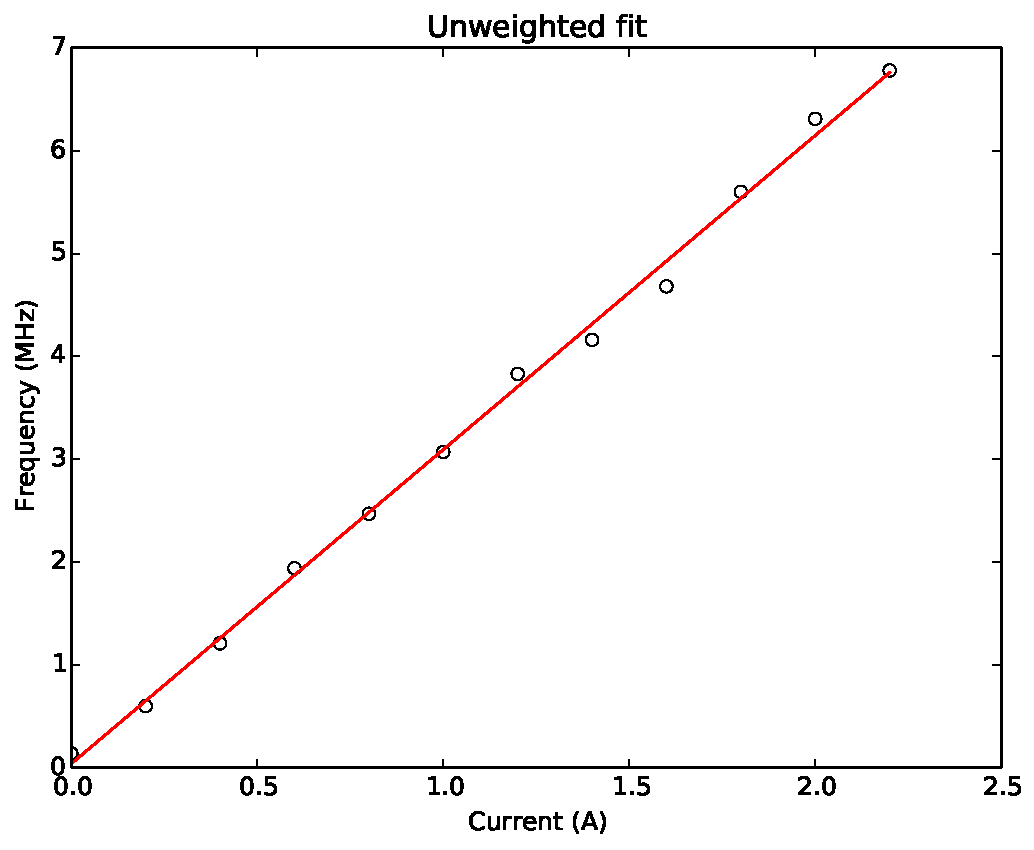
\includegraphics[width=\textwidth]{figures/problem5_1.pdf}
    \end{minipage}
    \hspace{0.5cm}
    \begin{minipage}[t]{0.45\textwidth}
        \centering
        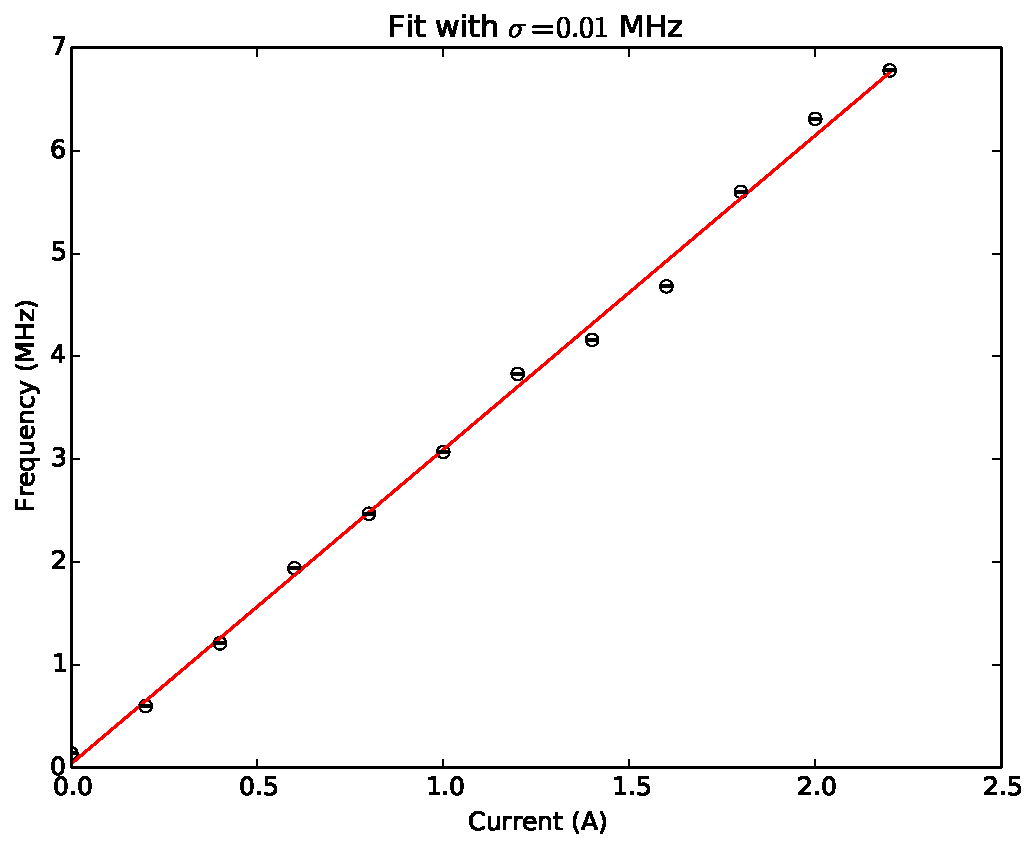
\includegraphics[width=\textwidth]{figures/problem5_2.pdf}
    \end{minipage}
    \begin{minipage}[t]{0.45\textwidth}
        \centering
        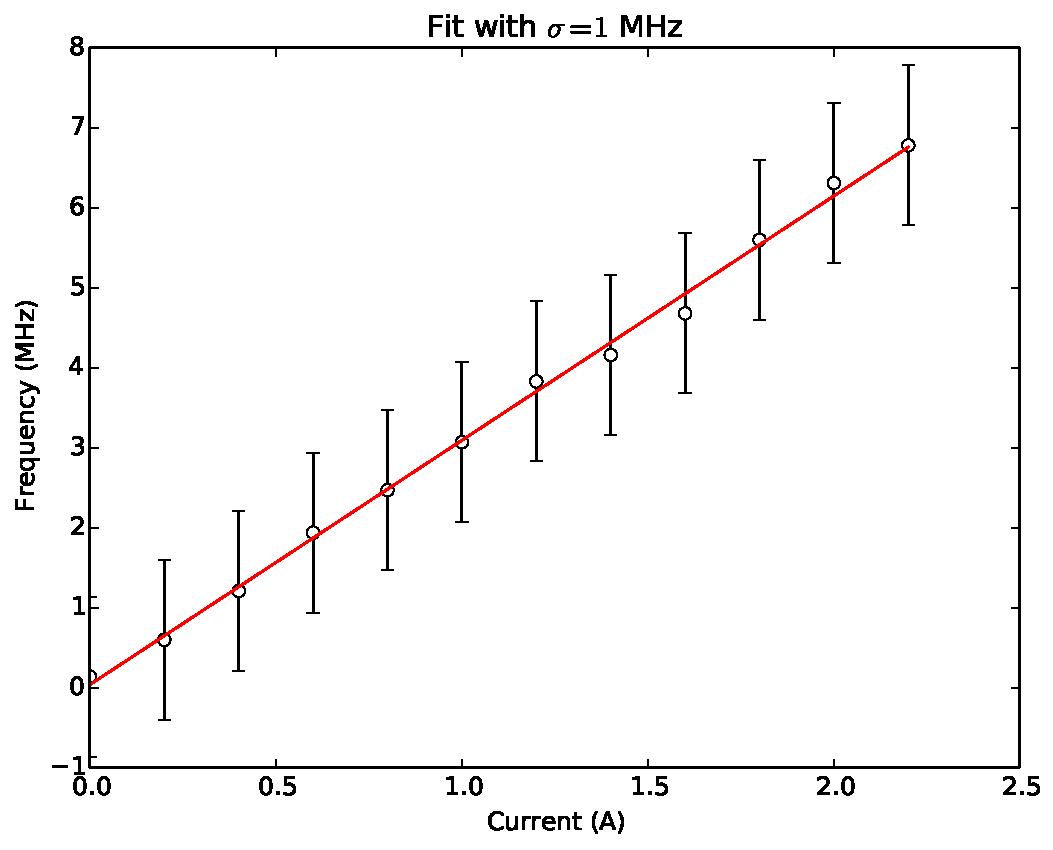
\includegraphics[width=\textwidth]{figures/problem5_3.pdf}
    \end{minipage}
    \hspace{0.5cm}
    \begin{minipage}[t]{0.45\textwidth}
        \centering
        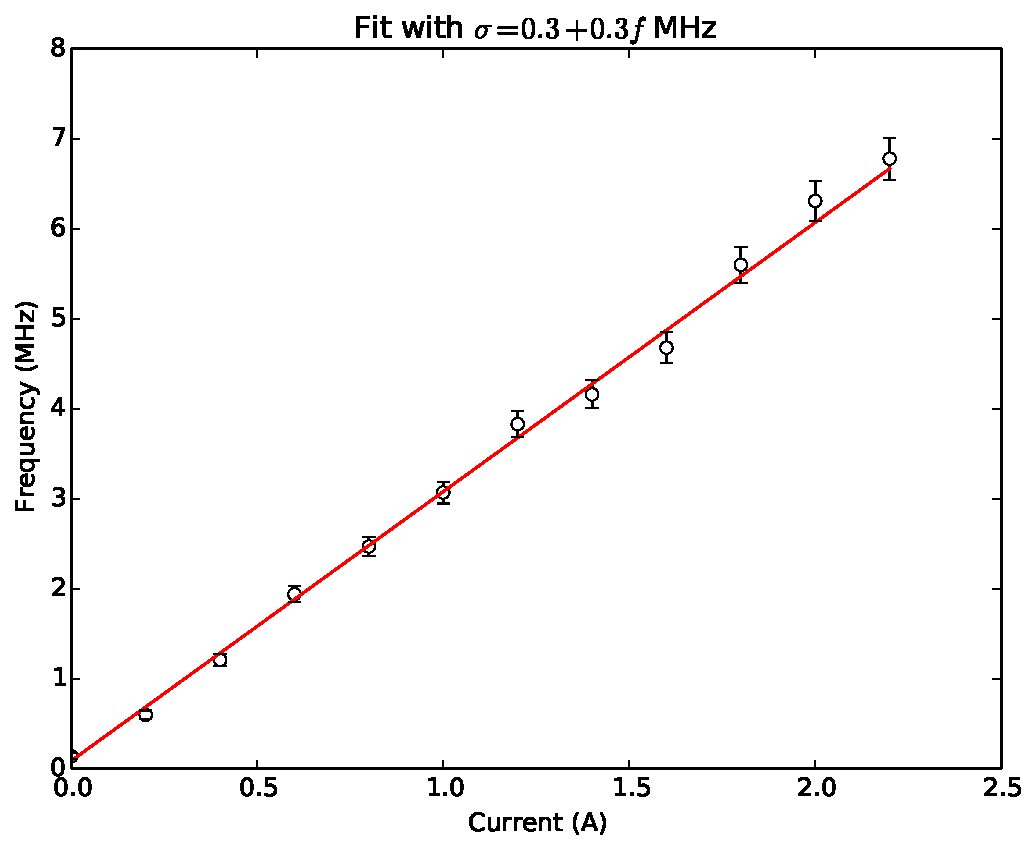
\includegraphics[width=\textwidth]{figures/problem5_4.pdf}
    \end{minipage}
    \caption{All examples on linear least squares fitting for the sample optical
    pumping data.}
    \label{optical}.
\end{figure}

\section*{Problem 6}

\begin{enumerate}
\item Before computing the mean of the distribution, the normalization must be
    verified, else the mean could possibly be incorrect. The distribution
    $e^{-x}$ is already normalized.
    \begin{displaymath}
        \int_0^\infty e^{-x}dx = 1
    \end{displaymath}
    The mean of the distribution is straightforward to compute.
    \begin{displaymath}
        \langle x \rangle = \int_0^\infty x e^{-x} dx = 1
    \end{displaymath}
    The variance of the distribution can be computed as such:
    \begin{displaymath}
        \sigma^2 = \int_0^\infty \left(x - \langle x \rangle\right)^2 e^{-x} dx
        = \int_0^\infty \left(x - 1\right)^2 e^{-x} dx = 1
    \end{displaymath}
\item Any measured $\left(x_i, y_i\right)$ will have some associated error
    $\sigma_i$ with it. When creating a log histogram, the errors of the bins
    will not be symmetric. Consider a histogram bin value of $y_i + \sigma_i$.
    The logarithm of this bin will be
    \begin{displaymath}
        f_i = \log\left(y_i + \sigma_i\right) = \log\left(y_i\left(1 +
        \frac{\sigma_i}{y_i}\right)\right) = \log\left(y_i\right) +
        \log\left(1 + \frac{\sigma_i}{y_i}\right) = \log\left(y_i\right) +
        \delta f_i^+
    \end{displaymath}
    Similarly, for a negative error $y_i - \sigma_i$, the logarithm will be
    \begin{displaymath}
        f_i = \log\left(y_i - \sigma_i\right) = \log\left(y_i\left(1 -
        \frac{\sigma_i}{y_i}\right)\right) = \log\left(y_i\right) +
        \log\left(1 - \frac{\sigma_i}{y_i}\right) = \log\left(y_i\right) -
        \delta f_i^-
    \end{displaymath}
    The errors $\delta f_i^\pm$ can be further investigated by considering their
    Taylor expansions.
    \begin{equation}
        \delta f_i^+ = \log\left(1 + \frac{\sigma_i}{y_i}\right) =
        \sum_{n=1}^\infty \left(-1\right)^{n+1} \frac{1}{n}
        \left(\frac{\sigma_i}{y_i}\right)^n
        \label{logerrp}
    \end{equation}
    \begin{equation}
        \delta f_i^- = -\log\left(1 + \frac{\sigma_i}{y_i}\right) =
        \sum_{n=1}^\infty \frac{1}{n} \left(\frac{\sigma_i}{y_i}\right)^n
        \label{logerrm}
    \end{equation}
    Due to the alternating sum in \eqref{logerrp}, it can be seen that
    $\delta f_i^- > \delta f_i^+$. If only the first terms in the Taylor series
    \eqref{logerrp} and \eqref{logerrm} are considered, it may appear that
    $\delta f_i^\pm$ are equal, but approximation that will only be true when
    $\sigma_i \ll y_i$.
\item Since $\log E_0 = 2.1 \pm 0.5$, the value for $E_0$ and the errors on
    $E_0$ are $E_0 = e^{2.1} \pm \delta E_0^\pm$, where $\delta E_0^+ \neq
    \delta E_0^-$. The errors on $E_0$ can be solved using \eqref{logerrp} and
    \eqref{logerrm} to get $\delta E_0^+ = E_0 \left(e^{\delta f} - 1\right)$
    and $\delta E_0^- = E_0 \left(1 - e^{-\delta f}\right)$, where $\delta f =
    0.5$. Applying all of this gets $E_0 = 8.17$, $\delta E_0^+ = 5.30$, and
    $\delta E_0^- = 3.21$. If the error was small, then the first term in the
    Taylor expansions of \eqref{logerrp} and \eqref{logerrm} could be used to
    get $\delta E_0$, but 0.5 is definitely not small compared to 2.1.
\end{enumerate}

\end{document}
